\section{Crittografia a chiave Privata (simmetrica)}

\begin{figure}[H]
    \centering
    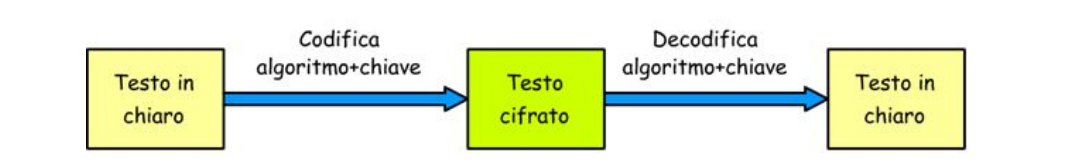
\includegraphics[width=\textwidth, keepaspectratio]{capitoli/crittografia/imgs/privata.png}
    \caption{Esempio del funzionamento della Crittografia Simmetrica.}
\end{figure}

La codifica e la decodifica sono eseguite dagli algoritmi crittografici assieme
ad una chiave che è la
stessa per entrambi i procedimenti. Tale chiave pertanto dovrà essere condivisa
tra le parti della
comunicazione. La segretezza, l'autenticazione e l'integrità dipendono dalla
segretezza della chiave.
Un sistema crittografico a chiave simmetrica molto conosciuto è il
\textbf{DES} ideato nel 1976 dalla IBM,
tuttora usato per cifrare files nei personal computer.
Questo sistema utilizza una chiave di 56 bit
(256 possibili chiavi).